\chapter{Introduction}
\label{chap:introduction}

\section{Techniques de mesure, métrologie, analyse des données}

En ingénierie, et dans toutes les branches scientifiques, les informations sur les systèmes physiques, construits par l'humain, ou naturels, sont obtenues par des \textbf{mesures}. deux questions essentielles se posent alors à l'expérimentateur:
\begin{enumerate}
    \item comment mesurer de la manière la plus juste possible,
    \item et comment déduire, des mesures brutes, l'information recherchée ?
\end{enumerate}
La première partie est du domaine de ce que nous pouvons nommer les \textbf{techniques de mesures}, accompagnée des règles de la \textbf{métrologie}. La seconde partie constitue le vaste domaine de \textbf{l'analyse des données}. Dans ce cours, nous traiterons tout d'abord des techniques des mesures, logiquement suivies de la présentation des techniques d'analyse de données.

\section{Utilité de la métrologie}

Les techniques de mesure ont recours à la métrologie, terme qui se traduit, au sens étymologique, par \textless\textless\ science de la mesure\ \textgreater\textgreater. Avant d'entrer dans le vif du sujet, à savoir les techniques de mesure, il est donc nécessaire de bien comprendre quels sont les défis résolus par la métrologie.

La métrologie s'intéresse traditionnellement à la détermination de caractéristiques (appelées grandeurs) qui peuvent être fondamentales comme par exemple une longueur, une masse, un temps, ou dérivées de grandeurs fondamentales comme par exemple une surface, une vitesse (notons que dans beaucoup de domaines, comme celui des essais des matériaux, la médecine ... il existe des unités spécialisées qui n'ont pas de lien forcément direct avec les unités fondamentales ci-dessus, mais qui sont néanmoins parfaitement définies).

Quoi qu'il en soit, mesurer une grandeur physique consiste à lui attribuer une valeur quantitative en prenant pour référence une grandeur de même nature appelée unité. Dans le langage courant des métrologues, on entend souvent dire \textless\textless\ mesurer c'est comparer\ \textgreater\textgreater.

\begin{figure}[ht]
    \centering
    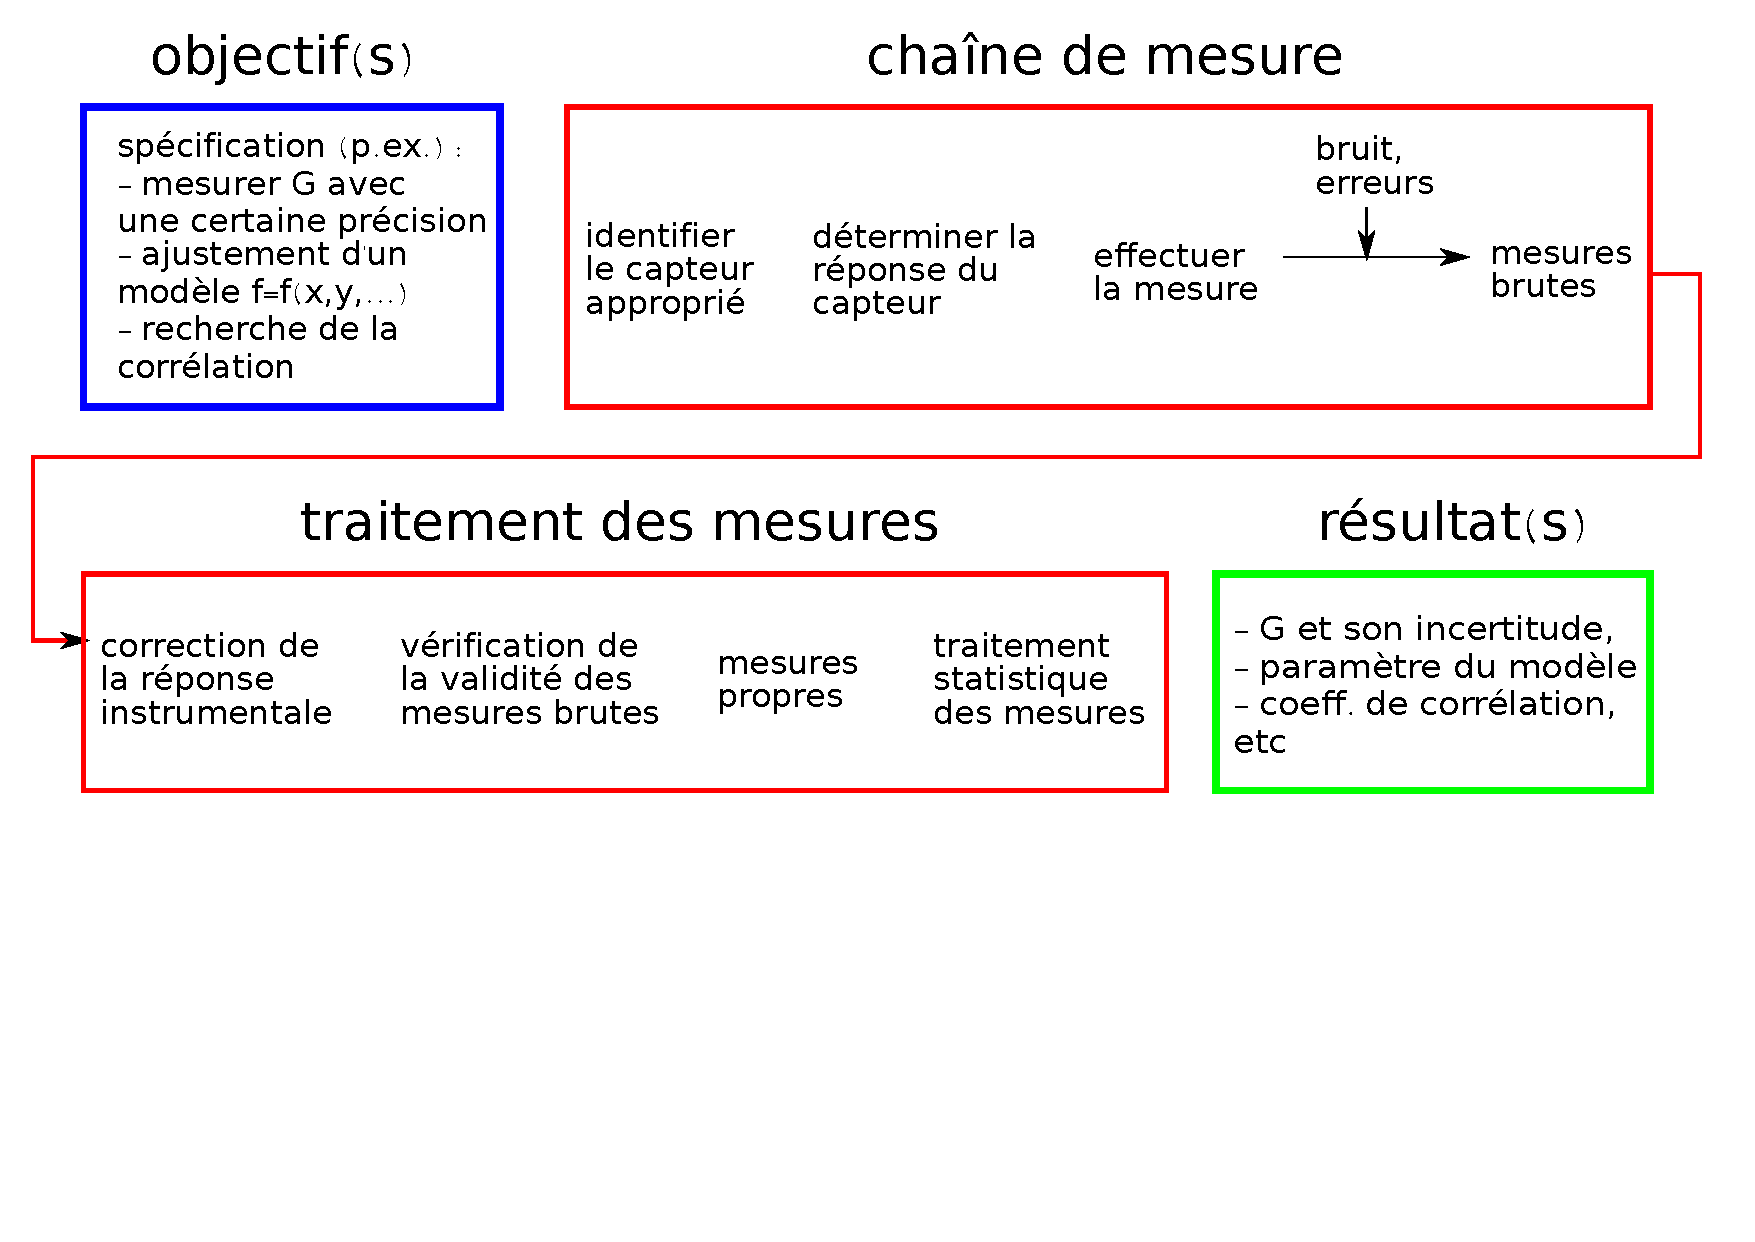
\includegraphics[width=0.9\textwidth]{assets/figures/flowChartTechMes.pdf}
    \caption{Techniques de mesure et traitement des données: les étapes clés.}
    \label{fig:flowchartTechMes}
\end{figure}
Les résultats des mesures servent à prendre des décisions dans de nombreux domaines, tels que:

\begin{itemize}
    \item validation d'une hypothèse scientifique,
    \item acceptation d'un produit (conformité à une exigence),
    \item réglage d'un paramètre dans le cadre du contrôle d'un procédé de fabrication,
    \item protection de l'environnement,
    \item définition des conditions de sécurité d'un produit ou d'un système.
\end{itemize}

L'ensemble de ces décisions concourt à la qualité des produits ou des services: on peut quantifier (ou caractériser) la qualité d'un résultat de mesure grâce à son incertitude.
En effet sans incertitude les résultats de mesure ne peuvent plus être comparés:

\begin{itemize}
    \item soit entre eux (essais croisés),
    \item soit par rapport à des valeurs de référence spécifiés dans une norme ou une spécification (conformité d'un produit).
\end{itemize}

Le diagramme de la figure  ~\ref{fig:flowchartTechMes} représente les différentes étapes nécessaires à la réalisation d'un système de mesure, depuis l'acquisition au traitement des mesures. C'est sur cette base que les chapitres ont été définis:

\begin{description}
    \item[Chapitre \ref{chap:introduction}] Introduction
    \item[Chapitre \ref{chap:si}] Le système international d'unités
    \item[Chapitre \ref{chap:measurement-chain}] La chaîne de mesure
    \item[Chapitre \ref{chap:measurement-chain-modelisation}] Modélisation de la chaîne de mesure
    \item[Chapitre \ref{chap:sensors}] Capteurs
\end{description}

La 2e partie traite de l'analyse des données:

\begin{description}
    \item[Chapitre \ref{chap:measurements}] La mesure et sa représentation
    \item[Chapitre \ref{chap:measurements-stochastic}] La mesure vue comme une variable aléatoire. Distributions usuelles des
          variables aléatoires.
    \item[Chapitre \ref{chap:measurements-multidimentional}] Mesures multidimensionnelles, corrélations, budget d'erreur
    \item[Chapitre \ref{chap:model-adjustment}] Ajustement d'un modèle sur une série de mesures
\end{description}

\textbf{A la fin de ce cours, vous devriez être capable de concevoir un système de mesure d'une grandeur physique donnée, et de traiter les données enregistrées pour en tirer les informations désirées.}
